%%
%
% ARQUIVO: cap-02.tex
%
% VERSÃO: 1.0
% DATA: Maio de 2017
% AUTOR: Carla Cosenza, Matheus Mello, Rebeca Reis
% 
%  Arquivo tex de exemplo de capítulo do documento de Projeto de Fim de Curso.
%
% ---
% DETALHES
%  a. todo capítulo deve começar com \chapter{•}
%  b. usar comando \noindent logo após \chapter{•}
%  c. citações para referências podem ser
%       i. \citet{•} para citações diretas (p. ex. 'Segundo Autor (2015)...'
%       ii. \citep{•} para citações indiretas (p. ex. '... (AUTOR, 2015)...'
%  d. notas de rodapé devem usar dois comandos
%       i. \footnotemark para indicar a marca da nota no texto
%       ii. \footnotetext{•}, na sequência, para indicar o texto da nota de rodapé
%  e. figuras devem seguir o exemplo
%       i. devem ficar no diretório /img e devem ser no formato EPS
%  f. tabelas devem seguir o exemplo
%  g. figuras e tabelas podem ser colocadas em orientação landscape
%       i. figuras: usar \begin{sidewaysfigure} ... \end{sidewaysfigure}
%                   em vez de \begin{figure} ... \end{figure}
%       ii. tabelas: usar \begin{sidewaystable} ... \end{sidewaystable}
%                    em vez de \begin{table} ... \end{table}
%  h. toda figura e tabela deve ser referenciada ao longo do texto com \ref{•}
% ---
%%

\chapter{Projeto e especificação do sistema}
\noindent

Além de seus respectivos fontes, 3 artefatos binários foram criados: hac, bfi e expander. 

\section{hac}

hac é o compilador de Headache para brainfuck. 

\begin{figure}[h]
    \centering
	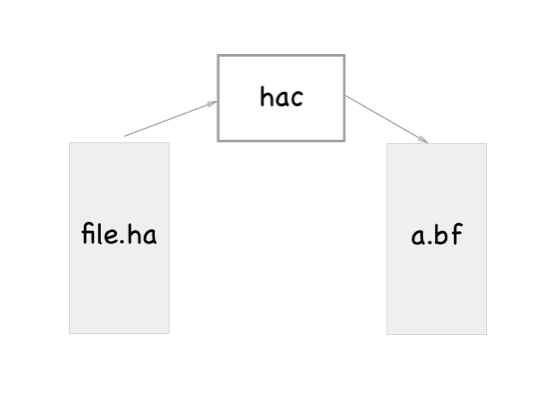
\includegraphics[]{TD/img/hac.png}
	\caption{Esquema simples sobre o hac}
	\label{hac}
\end{figure}

A utilização usual do hac é descrita como:

\begin{verbatim}
    ./hac [opção] file.ha
\end{verbatim}

file.ha é o arquivo source em Headache (.ha) a ser convertido em brainfuck. 

O resultado é sempre salvo em um arquivo nomeado a.bf.

Antes do arquivo source.ha, poderá vir uma opção de interrupção do fluxo de controle.

São elas: 

\begin{itemize}
    \item -lex: roda apenas o analisador léxico.
    \item -syntax: diz se o programa fornecido no input pertence à gramática de Headache.
    \item -tree: Exibe a AST gerada a partir do programa fornecido.
    \item -check: Checa erros e alertas sem compilar o programa.
    \item -noBin: Não executa o interpretador interno após a compilação.
\end{itemize}

Se nenhum programa for fornecido ao hac, ele entrará no "modo interativo", isto é, esperará o programa pela entrada padrão.

Além disso, o hac poderá receber o parâmetro de otimização -O0 ou -O1. Este parâmetro pode vir antes ou depois dos outros parâmetros. Se o parâmetro for -O0, o hac não efetuará nenhuma otimização na AST. Caso -O1 seja fornecido, o hac aplicará otimizações de constantes em tempo de compilação. Isso é feito simplificando operações de constantes na AST. 

Por exemplo: com -O1 expressões como "@1+1+1;" são transformadas em "@3;" na própria AST. 

-O2 transforma operações como "a = a + 3;" em "a+=3", que em brainfuck é apenas "goto(a); +++". Incremento e decremento são nativos em brainfuck, e muito mais rápidos que operações de adição e atribuição, resultando em uma otimização genuína. Essa feature não está corretamente implementada, contudo.

Além disso, o hac também tem as opções --help e --version para a conveniência do usuário.

O hac foi projetado de forma similar ao mongaComp (projeto da disciplina de compiladores). Os códigos estão modularizados de acordo com o seguinte fluxo de execução:

\begin{figure}[h]
    \centering
	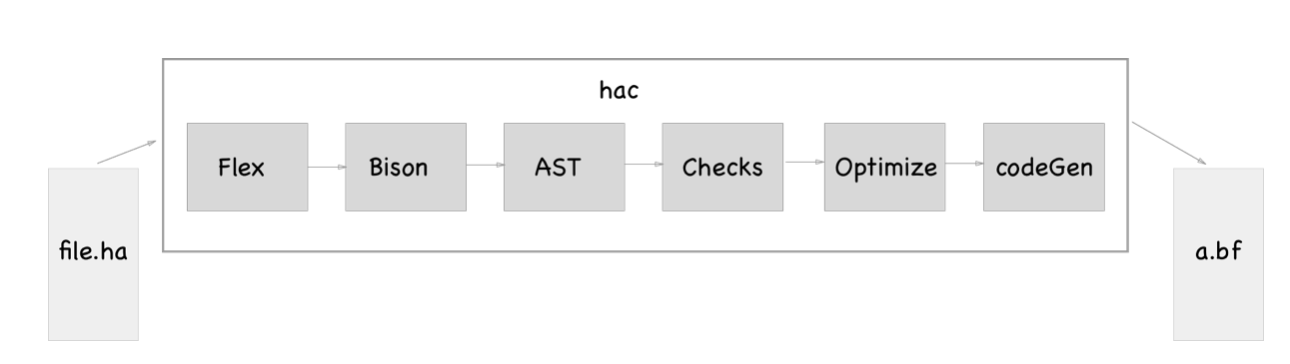
\includegraphics[width = 15cm]{TD/img/esquematicoHac.png}
	\caption{Esquema de funcionamento do hac}
	\label{esquematicoHac}
\end{figure}

O código de input é transformado em tokens; os tokens são avaliados pela gramática, gerando a AST. A AST é checada, tipada. É otimizada, se a opção estiver habilitada e depois é gerado o código output.

bfi (Brainfuck Interpreter) é a versão standalone interpretador de brainfuck utilizado para testes. Uma regra no makefile permite ativar \#ifdef que compila o arquivo testbfi.c com uma main, gerando o bfi. 

\begin{figure}[h]
    \centering
	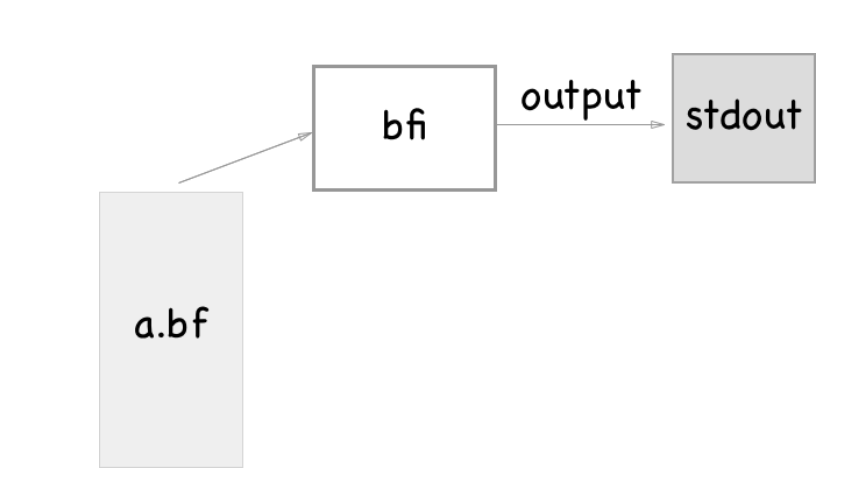
\includegraphics[width = 10cm]{TD/img/bfi.png}
	\caption{Esquema simples sobre bfi}
	\label{bfi}
\end{figure}

\section{bfi}

o bfi é usado da seguinte forma:

\begin{verbatim}
    ./bfi arquivo.bf [-extra]
\end{verbatim}

Isso executa o arquivo brainfuck e imprime na saída padrão. Se o arquivo brainfuck tiver os whiles desemparelhados (instruções '[' e ']'), ele não executa o programa, porém exibe uma mensagem de erro. 

Se a opção -extra for fornecida, o bfi interpreta cada ocorrência do caractere '@' como instrução de debug. Ao encontrar o '@', o bfi exibe o estado atual da memória do interpretador naquele momento da execução. 

A opção "-extra" do bfi faz parte das ferramentas de debug de Headache e está relacionada com a instrução de debug do hac. O comando "\%;"  faz com que o hac gere '@' para que se ative o print da memória naquele momento da execução.

Essas instruções não fazem parte do padrão de brainfuck e portanto só são acionados se os respectivos parâmetros forem fornecidos.

\section{expander}

O expander é um programa para executar extensão de bitwidth de programas brainfuck. Por extensão de bitwidth este documento se refere a transformar um programa em brainfuck de 8 bits em um programa com 16 bits, 32 bits quando executado num interpretador de brainfuck de 8 bits. Isso é obtido por transformar cada instrução em uma sequência maior de instruções. 

\begin{figure}[h]
    \centering
	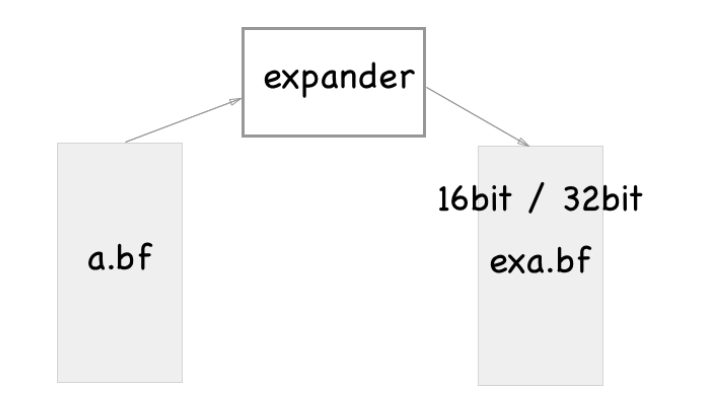
\includegraphics[width = 7cm]{TD/img/expander.png}
	\caption{Esquema simples sobre o expander}
	\label{expander}
\end{figure}

É assim que Headache implementa inteiros de mais de 8 bits. (shorts e ints) .

O expander é utilizado da seguinte forma:

./expander sourcepath [mode]: recebe o path do arquivo brainfuck como input 

ou

./expander -p "source" [mode] : recebe o input entre aspas

ou

./expander -i [mode] : ativa o modo interativo (recebe o input na entrada padrão)

O expander sempre imprime o resultado na saída padrão. 

O parâmetro opcional mode é um inteiro pertencente a {0,1,2}. Cada número representa uma transformada a ser aplicada nas instruções. Os modos 0 e 1 são estratégias diferentes para expandir x2 bits e o modo 2 é para expandir x4 bits.

Um exemplo para entender o funcionamento do expander é:

\begin{verbatim}
    expanding.ha
    void main(){
        byta a;
        a = 200;
        a = a + a;
        @a;@"\n";
    }
    ./hac expanding.ha 
    ./bfi a.bf
    144
\end{verbatim}

Porém se aplicarmos:

\begin{verbatim}
    ./expander a.bf > exa.bf
    ./bfi exa.bf
    400
\end{verbatim}

Ou seja, programa assume o comportamento de:

\begin{verbatim}
    void main(){
        short a;
        a = 200;
        a = a + a;
        @a;@"\n";
    }
\end{verbatim}

Infelizmente, ainda não é possível ao hac expandir apenas as instruções que lidem com shorts, porém, o hac consegue sim compilar programas que tenham shorts: Ao detectar um tipo com mais de 8 bits, uma variável é modificada para saber a quantidade de expansão necessária na main.c; O programa é compilado como se tudo fossem bytes, e  ao final da compilação, o output é expandido.

Os arquivos fontes do expander possuem a macro standalone assim como o bfi. Eles são compilados junto ao hac para que as funções do expander sejam automaticamente chamadas se o hac detectar shorts ou ints no seu input. Isso o torna capaz de gerar output em brainfuck de 8 bits capaz de 16 ou 32 bits.

Contudo, com o uso do expander como programa standalone é perfeitamente possível que um programa feito somente com shorts seja obtido expandido de um programa feito somente com bytes. Inclusive programas brainfuck não gerados pelo hac.

Nenhuma das soluções citadas anteriormente lida com inteiros acima de 8 bits. Até o conhecimento do autor desse projeto, isso é uma exclusividade de Headache.

\section{bfalgoConverter}

Há ainda o bfalgoConverter, mencionado anteriormente. Ele permite traduzir os algoritmos publicados na Brainfuck Algorithms diretamente para chamadas da função bfalgo() (que Headache usa para codificar os algoritmos na hora de gerar o código output).

Como a Brainfuck Algorithms continua a ser atualizada, o bfalgoConverter ajudará futuros colaboradores a adicionar novas features e melhorar as existentes.

\begin{figure}[h]
    \centering
	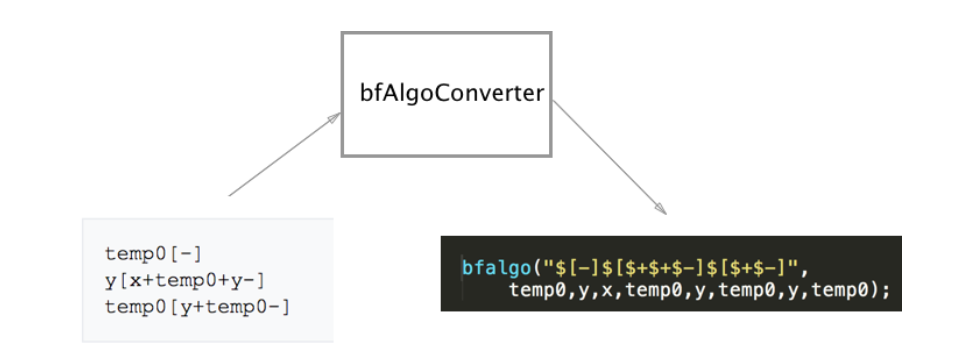
\includegraphics[]{TD/img/bfalgo.png}
	\caption{Esquema do bfalgoConverter}
	\label{Bfalgo}
\end{figure}